\section{How to conduct nesting experiment} \label{sec:nest_exp}
%====================================================================================

``Nesting'' is the method for settings multiple computational domains overlapping one another in a nested structure. Figure \ref{fig_nestsample} shows an example of nesting using three domains. An outer domain is configured to be wider with coarser resolution to express larger-scale phenomena, while an inner domain is set narrower with finer resolution to represent smaller-scale phenomena. The result calculated in the outer domain is used for the boundary condition for the inner domain.
%Hereinafter, the domain that sends data is called the ``parent domain'' and that which receives data is called the ``child domain.''
Hereinafter, the outer domain that sends data is called the ``parent domain'' and the inner domain which receives data is called the ``child domain.''

Nesting methods are categorized as follows:
\begin{itemize}
\item Execution procedure
\begin{description}
 \item[Online nesting]\mbox{}\\
The computations in the parent and child domains are simultaneously conducted by exchanging information.
 \item[Off-Line nesting]\mbox{}\\
Following the computation of the parent domain, the initial and boundary conditions of the child domain are formulated, and then the child domain is computed.
\end{description}
\item Method of data exchange
\begin{description}
 \item[One-way nesting]\mbox{}\\
The parent domain sends data to the child domain. The latter does not send data to the former. Thus, data flow is one way. The results of the parent domain are not affected by those of the child domain.
 \item[Two-way nesting]\mbox{}\\
The parent domain sends data to the child domain. The former also receives data from the latter. Thus, the calculations of the domains influence each other. Although this method can be applied in the case of online nesting, it has not yet been implemented in {\scalerm} v{\version}.
\end{description}
\end{itemize}

The difference between online and offline nestings lie in the update frequency of providing data from the parent domain to the child domain. In an online nesting experiment, the boundary conditions of the child domain are updated at every time step ($\Delta t$) of the parent domain. In an offline nesting experiment, the update interval depends on the output interval of the history file in the calculation of the parent domain. 

Regardless of whether the nesting is online or offline, the ratio of the grid interval of the parent domain to that of the child domain  ($\mathrm{DX}_{\mathrm{d01}}/\mathrm{DX}_{\mathrm{d02}}$) is not limited in terms of code implementation. However, there is the possibility of degradation in the physical performance of the results of calculations if the ratio is too high. In \scalerm, it is recommended that this ratio be equal to or lower than 5.

In this section, the configuration files for the parent and child domains
are denoted by \verb|***.d01.conf| and \verb|***.d02.conf|, respectively.

\begin{figure}[t]
\begin{center}
  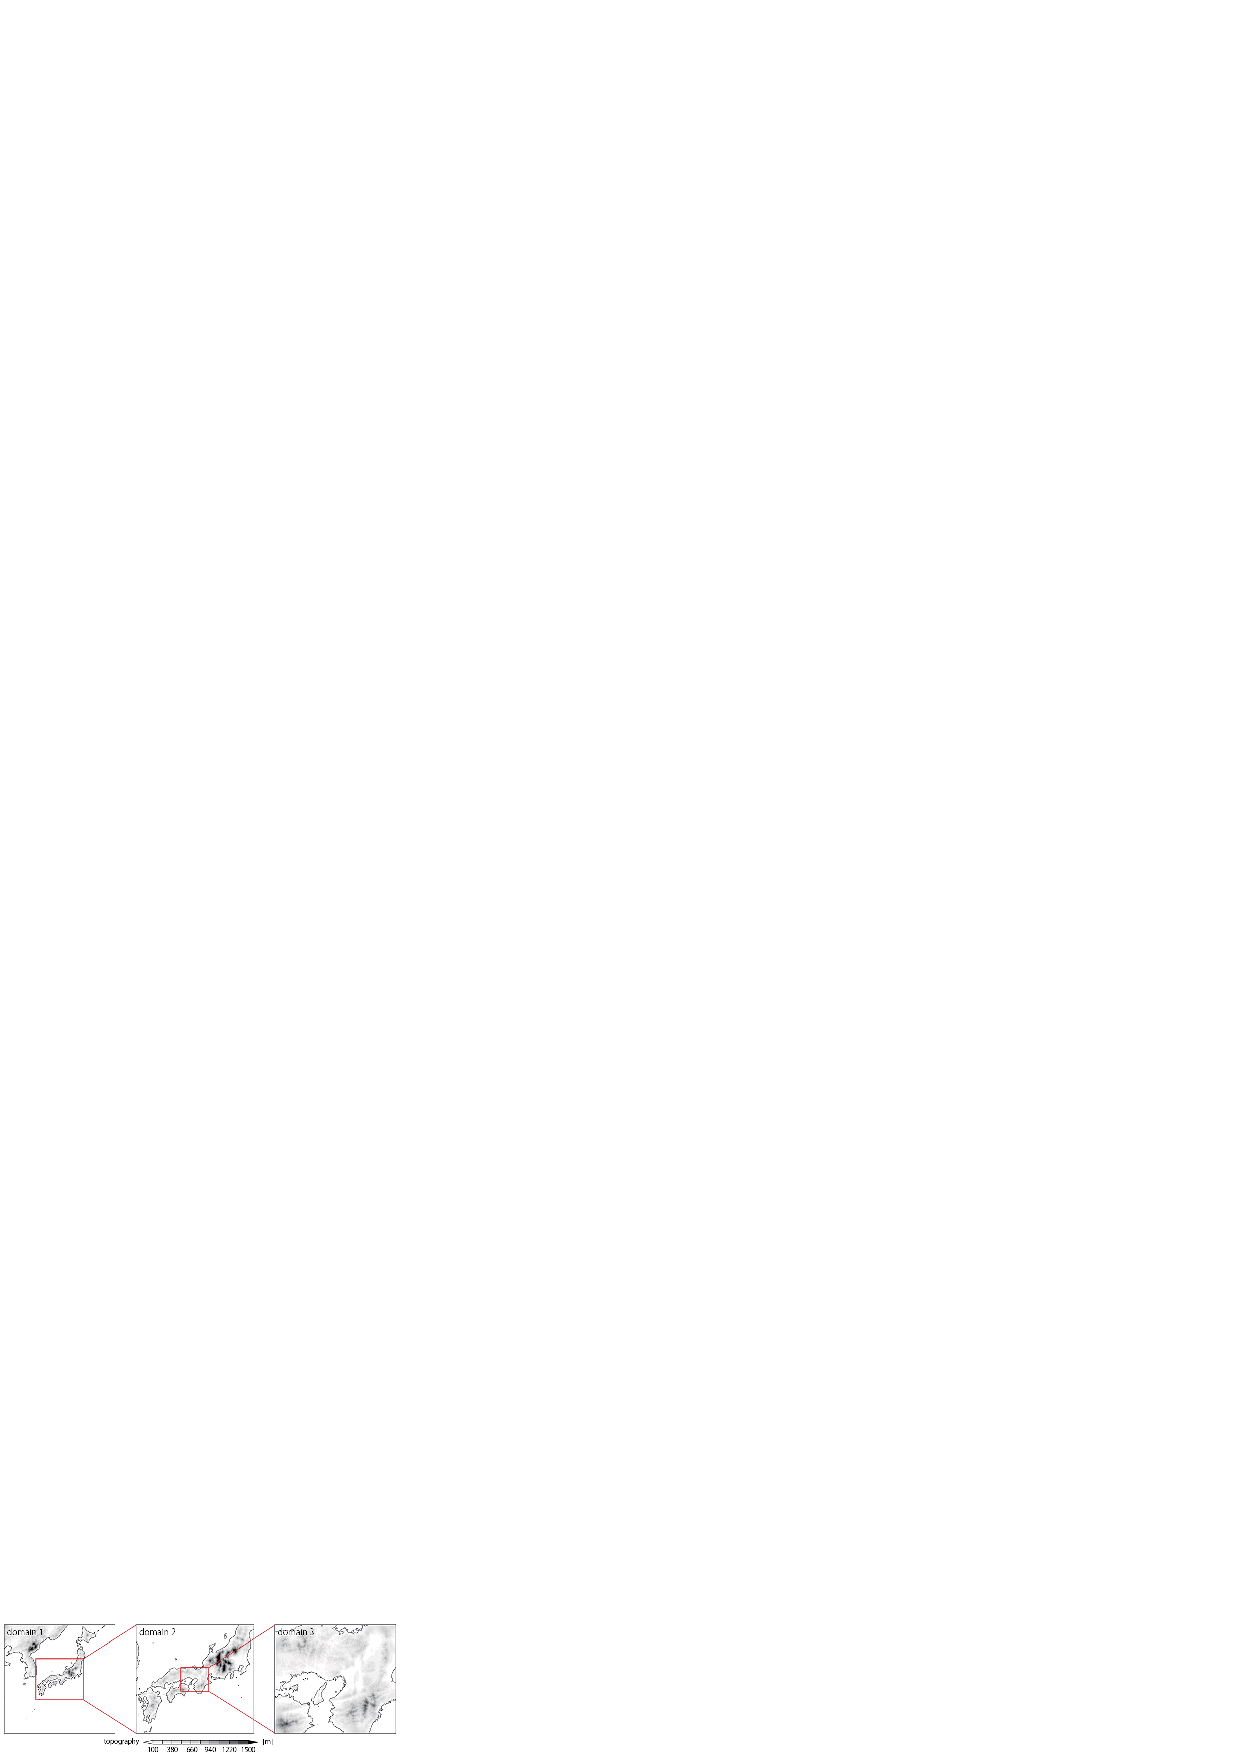
\includegraphics[width=1.0\hsize]{./../../figure/nesting_sample.pdf}\\
  \caption{An example of domain nesting targeting the western area of Japan.
    Domain 1 is the outermost domain and domain 3 the innermost.
    The red rectangle and lines represents the domain’s location and its relations with other domains.
    The horizontal grid spacings are 7.5 km, 2.5 km, and 0.5 km for Domains 1, 2, and 3, respectively.
  }
  \label{fig_nestsample}
\end{center}
\end{figure}



